% Chapter Template

\chapter{Stochastic Collocation for Generalized Polynomial Chaos Method} % Main chapter title

\label{ch:methods scgpc} % Change X to a consecutive number; for referencing this chapter elsewhere, use \ref{ChapterX}

\lhead{Chapter 3. \emph{Methods: SCgPC}} % Change X to a consecutive number; this is for the header on each page - perhaps a shortened title

%----------------------------------------------------------------------------------------
%	SECTION: INTRO
%----------------------------------------------------------------------------------------

\section{Introduction}
Expanding beyond the traditional uncertainty quantification methods of MC, Grid, and LHS sampling, there are more
advanced methods that are very efficient in particular applications.
Generalized polynomial chaos (gPC) expansion methods, for example, interpolate the model as a combination of
polynomials of varying degree in each dimension of the input space.  There are several advantages to expanding
in polynomials \cite{xiu}.  First, orthonormal polynomials have means and standard deviations that are trivial to calculate
analytically, even for computer algorithms.  Second, the resulting polynomial expansion is an
inexpensive surrogate that can be used in place of the original model.  Polynomials are generally inexpensive
to evaluate, especially in comparison to complex solvers.  Third, the unknowns in the expansions
are scalar coefficients, which can often be efficiently calculated through numerical integration.

Originally Wiener
proposed expanding models in Hermite polynomials for Gaussian-normal distributed input variables \cite{wiener}.  Askey and
Wilson generalized Hermite polynomials to include Jacobi polynomials, including Legendre and Laguerre
polynomials \cite{Wiener-Askey}.  Xiu and Karniadakis combined these concepts to perform gPC expansions for a 
range of Gaussian-based distributions with corresponding polynomials,
including Legendre polynomials for uniform distributions, Laguerre polynomials for Gamma distributions, and
Jacobi polynomials for Beta distributions, in addition to Hermite polynomials for normal distributions
\cite{xiu}.  More information on how to use these distributions and polynomials is contained in Appendix
\ref{apx:quads dists}.

In each of these cases, a probability-weighted
integral over the distribution can be cast in a way that the corresponding polynomials are orthogonal over the
same weight and interval.  These chaos Wiener-Askey polynomials were used by Xiu and Karniadakis to develop
the generalized polynomial chaos expansion method (gPC), including a transformation for applying the same
method to arbitrary distributions (as long as they have a known inverse CDF) \cite{xiu}.  Two significant
methodologies have branched from gPC applications.  The first makes use of Lagrange polynomials to expand the
original function or simulation code \cite{SCLagrange}, as Lagrange polynomials can be made orthogonal over the same domain as the
distributions; the other uses the Wiener-Askey polynomials \cite{xiu}.  We consider the latter in this work.

We consider a simulation code that produces a quantity of interest $u(Y)$ whose
arguments are the uncertain, distributed input
parameters $Y=(y_1,\ldots,y_n,\ldots,y_N)$.  A particular realization $\omega$ of $y_n$ is expressed by
$y_n(\omega)$, and a single realization of the entire input space results in a solution to the response as
$u(Y(\omega))$.  We acknowledge obtaining a realization of $u(Y)$ may take considerable computation time and
effort, and may be solved nonlinearly.  There also may be other input parameters that
contribute to the solution of $u(Y)$ but have no associated uncertainty; we neglect these, as our interest 
is in the uncertainty space.  All parameters without uncertainty are held at their nominal values.
In addition, it is possible that the quantity of interest $u(Y)$ is an integrated quantity or some norm of a
value that is temporally or spatially distributed. We restrict $u(Y(\omega))$ to a single scalar
output, but the same principles apply to a multidimensional response.  Further, a quantity of interest may be
time-dependent in a transient simulation.  In this case, the gPC expansion can be constructed at several selected points
in time throughout the simulation, which can then be interpolated between.  In effect, the polynomial
coefficients become time-dependent scalar values.  This will be discussed and demonstrated in Chapter \ref{ch:timedep}. 
For now, we consider a static case with no time dependence.

We expand $u(Y)$ in orthonormal multidimensional polynomials $\Phi_k(Y)$, where $k$ is a multi-index tracking
the polynomial order in each axis of the polynomial Hilbert space, and $\Phi_k(Y)$ is constructed as
\begin{equation}
  \Phi_k(Y) = \prod_{n=1}^N \phi_{k_n}(Y_n),
\end{equation}
where $\phi_{k_n}(Y_n)$ is a single-dimension Wiener-Askey orthonormal polynomial of order $k_n$ and
$k=(k_1,\ldots,k_n,\ldots,k_N)$, $k_n\in\mathbb{N}_0$.  For example, given $u(y_1,y_2,y_3)$, $k=(2,1,4)$
is the multi-index of the
product of a second-order polynomial in $y_1$, a first-order polynomial in $y_2$, and a fourth-order
polynomial in $y_4$. If $\phi$ were taken from monomials, this polynomial would be
\begin{equation}
  \phi_{(2,1,4)} = y_1^2\ y_2\ y_3^4.
\end{equation}
The gPC for $u(Y)$ using this notation is
\begin{equation}\label{eq:gPC}
  u(Y) \approx \sum_{k\in\Lambda(L)} u_k\Phi_k(Y),
\end{equation}
where $u_k$ is a scalar weighting polynomial expansion coefficient, sometimes called a polynomial expansion
moment. The polynomials used in the expansion are determined
by $\Lambda$, a set of chosen multi-indices, which can be selected in a variety of ways we will discuss in section
\ref{sec:index sets}.  In the limit
that $\Lambda$ contains all possible combinations of polynomials of any order, Eq. \ref{eq:gPC} is exact.
Practically, however, $\Lambda$ is truncated to some finite set of multidimensional polynomials.

We make use of orthonormal Wiener-Askey polynomials
\begin{equation}
  \int_\Omega \Phi_k(Y)\Phi_{\hat k}(Y) dY = \delta_{k\hat k},
\end{equation}
where $\Omega$ is the multidimensional domain of $Y$ and $\delta_{nm}$
is the Dirac delta.  We can isolate an expression for the polynomial expansion coefficients using the
properties of orthonormality.
We multiply both sides of Eq. \ref{eq:gPC} by
$\Phi_{\hat k}(Y)$, integrate both sides over the probability-weighted input domain, and sum over all $\hat k$
to obtain the coefficients $u_k$, sometimes referred to as polynomial expansion moments,
\begin{equation}
  u(Y) = \sum_{k\in\Lambda(L)} u_k\Phi_k(Y),
\end{equation}
\begin{equation}
  \int\limits_\Omega u(Y)\Phi_{\hat k}(Y) dY = \int\limits_\Omega u_{\hat k} \sum_{k\in\Lambda(L)}
           u_k\Phi_k(Y)\ dy,
\end{equation}
\begin{equation}
  \langle u(Y),\Phi_{\hat k}(Y)\rangle = \langle \Phi_{\hat k}(Y),\sum_{k\in\Lambda(L)}
           u_k\Phi_k(Y) \rangle,
\end{equation}
\begin{equation}
  \langle u(Y),\Phi_{\hat k}(Y)\rangle = \langle \Phi_{\hat k}(Y),\sum_{k\in\Lambda(L)}
           u_k\Phi_k(Y) \rangle,
\end{equation}
\begin{equation}
  \langle u(Y),\Phi_{\hat k}(Y)\rangle = \sum_{k\in\Lambda(L)} u_k \delta_{k,\hat k},
\end{equation}
\begin{equation}
  \langle u(Y),\Phi_{\hat k}(Y)\rangle = u_{\hat k} ,
\end{equation}
and swapping $\hat k$ for $k$ for convenience,
\begin{equation}\label{eq:polycoeff}
  u_k = \langle u(Y),\Phi_k(Y) \rangle,
\end{equation}
where we use the angled bracket notation to denote the probability-weighted inner product,
\begin{align}
  \langle f(Y),g(Y) \rangle &\equiv \int\limits_\Omega f(Y)g(Y) dY, \\
    &= \int\limits_a^b f(Y)g(Y)\rho(Y) dY.
\end{align}
When $u(Y)$ has an analytic form, these coefficients can be solved by direct integration; however, in general
numerical integration must be used instead.  While tools such as Monte Carlo integration can
be used to evaluate the integral, we can harness the properties of Gaussian quadratures because of the
probability weights, domain of integration, and the orthonormal polynomials.
This \emph{stochastic collocation} numerical integration method is discussed in section \ref{sec:stoch
coll}, and a discussion of the synergy between probability weights, domain of integration, and the 
orthonormal polynomials is included in Appendix \ref{apx:quads dists}.  Once the polynomial expansion 
coefficients $u_k$ are all obtained, the gPC expansion is complete.

\section{Polynomial Index Set Construction}\label{sec:index sets}
The chief concern in expanding a function in interpolating multidimensional polynomials is choosing appropriate polynomials to
make up the expansion.
There are many generic ways by which a polynomial set can be constructed.  Here we present three static
approaches: tensor
product, total degree, and hyperbolic cross.

In the tensor
product case, $\Lambda(L)$ contains all possible combinations of polynomial indices up to truncation order $L$ in each
dimension, as
\begin{equation}
  \Lambda_\text{TP}(L)=\Big\{\bar k=(k_1,\cdots,k_N): \max_{1\leq n\leq N}k_n\leq L \Big\}.
\end{equation}
The cardinality of this index set is $|\Lambda_\text{TP}(L)|=(L+1)^N$. For example, for a two-dimensional
input space ($N$=2) and truncation limit $L=3$, the index set $\Lambda_\text{TP}(3)$ is given in Table
\ref{tab:TP}, where the notation $(1,2)$ signifies the product of a polynomial that is first order in $Y_1$
and second order in $Y_2$.

\begin{table}[h]
  \centering
  \begin{tabular}{c c c c}
    (3,0) & (3,1) & (3,2) & (3,3) \\
    (2,0) & (2,1) & (2,2) & (2,3) \\
    (1,0) & (1,1) & (1,2) & (1,3) \\
    (0,0) & (0,1) & (0,2) & (0,3)
  \end{tabular}
  \caption{Tensor Product Index Set, $N=2,L=3$}
  \label{tab:TP}
\end{table}

It is evident there is some inefficiencies in this index set.  First, it suffers dramatically from the
\emph{curse of dimensionality}; that is, the number of polynomials required grows exponentially with
increasing dimensions.  Second, the total order of polynomials is not respected.  Assuming the contribution of
each higher-order polynomial is smaller than lower-order polynomials, the (3,3) term is
contributing sixth-order corrections that are likely smaller than the error introduced by ignoring
fourth-order corrections (4,0) and (0,4).  This leads to the development of the \emph{total degree} (TD) and
\emph{hyperbolic cross} (HC) polynomial index set construction strategies \cite{hctd}.

In TD, only multidimensional polynomials whose \emph{total} order are at most $L$ are permitted,
\begin{equation}
  \Lambda_\text{TD}(L)=\Big\{\bar k=(k_1,\cdots,k_N):\sum_{n=1}^N k_n \leq L \Big\}.
\end{equation}
The cardinality of this index set is $|\Lambda_\text{TD}(L)|={L+N\choose N}$ \cite{hctd}, which grows with increasing
dimensions much more slowly than TP.  For the same $N=2,L=3$ case above, the TD index set is given in Table
\ref{tab:TD}. 

\begin{table}[h]
  \centering
  \begin{tabular}{c c c c}
    (3,0) &       &       &       \\
    (2,0) & (2,1) &       &       \\
    (1,0) & (1,1) & (1,2) &       \\
    (0,0) & (0,1) & (0,2) & (0,3)
  \end{tabular}
  \caption{Total Degree Index Set, $N=2,L=3$}
  \label{tab:TD}
\end{table}

In HC, the \emph{product} of polynomial orders is used to restrict allowed polynomials in the index set.  This
tends to polarize the expansion, emphasizing higher-order polynomials in each dimension but lower-order
polynomials in combinations of dimensions, as
\begin{equation}
  \Lambda_\text{HC}(L)=\Big\{\bar k=(k_1,\ldots,k_N):\prod_{n=1}^N\qty(k_n+1) \leq L+1 \Big\}.
\end{equation}
The cardinality of this index set is bounded by $|\Lambda_\text{HC}(L)|\leq (L+1)(1+\log(L+1))^{N-1}$
\cite{hctd}. It
grows even more slowly than TD with increasing dimension, as shown in Table \ref{tab:HC} for $N=2,L=3$.

\begin{table}[h]
  \centering
  \begin{tabular}{c c c c}
    (3,0) &       &       &       \\
    (2,0) &       &       &       \\
    (1,0) & (1,1) &       &       \\
    (0,0) & (0,1) & (0,2) & (0,3)
  \end{tabular}
  \caption{Hyperbolic Cross Index Set, $N=2,L=3$}
  \label{tab:HC}
\end{table}

It has been shown that the effectiveness of TD and HC as index set choices depends strongly on the regularity
of the response \cite{hctd}.  TD tends to be most effective for infinitely-continuous response surfaces,
while HC is more effective for surfaces with limited smoothness or discontinuities.

\subsection{Anisotropy}
While using TD or HC to construct the polynomial index set combats the curse of dimensionality present in TP,
the polynomial set still grows swiftly with increasing dimension, and this continues to be an issue for problems 
of large dimensionality.  Another concept that can
be applied to mitigate this issue is index set anisotropy, or the unequal treatment of various dimensions.
In many models we expect different input dimensions to have different effective polynomial orders.  As defined
above, polynomial index sets are isotropic in dimension; anisotropy will cater to the unequal effective
polynomial orders in each dimension.
In this strategy, weighting factors $\alpha=(\alpha_1,\ldots,\alpha_n,\ldots,\alpha_N)$ are applied in each
dimension to allow additional polynomials in some dimensions and less in others.  This change adjusts the TD
and HC construction rules as follows,
\begin{equation}
  \tilde\Lambda_\text{TD}(L)=\Big\{\bar p=(p_1,\cdots,p_N):\sum_{n=1}^N \alpha_n p_n \leq 
  \frac{\qty|\vec\alpha|_1}{N} L \Big\},
\end{equation}
\begin{equation}
  \tilde\Lambda_\text{HC}(L)=\Big\{\bar p=(p_1,\cdots,p_N):\prod_{n=1}^N \qty(p_n+1)^{\alpha_n} \leq
  \qty(L+1)^{\qty|\vec\alpha|_1/N} \Big\}.
\end{equation}
where $|\alpha|_1$ is the one-norm of $\alpha$
\begin{equation}
  |\alpha|_1 = \sum_{n=1}^N \alpha_n.
\end{equation}
Considering the same case above ($N=2,L=3$), we apply weights $\alpha_1=5,\alpha_2=3$, and the resulting index
sets are Tables \ref{tab:aniTD} (TD) and \ref{tab:aniHC} (HC).

\begin{table}[h]
  \centering
  \begin{tabular}{c c c c c}
    (2,0) &       &       &       & \\
    (1,0) & (1,1) & (1,2) &       & \\
    (0,0) & (0,1) & (0,2) & (0,3) & (0,4)
  \end{tabular}
  \caption{Anisotropic Total Degree Index Set, $N=2,L=3$}
  \label{tab:aniTD}
\end{table}

\begin{table}[h]
  \centering
  \begin{tabular}{c c c c}
    (1,0) &       &       &       \\
    (0,0) & (0,1) & (0,2) & (0,3)
  \end{tabular}
  \caption{Anisotropic Hyperbolic Cross Index Set, $N=2,L=3$}
  \label{tab:aniHC}
\end{table}

There are many methods by which anisotropy weights can be chosen.  Often, if a problem is well-known to an 
analyst, it may be enough to use intuitive judgement to assign importance arbitrarily.  Otherwise, a smaller
uncertainty quantification solve can be used to roughly determine sensitivity coefficients (such as Pearson
coefficients), and the inverse of those can then be applied as anisotropy weights.  Sobol sensitivity coefficients
\cite{gfunc} could also serve as a basis for these weights.
A good choice of anisotropy weight can greatly speed up convergence; however, a
poor choice can slow convergence considerably, as computational resources are used to resolve low-impact
polynomials.


\section{Polynomial Expansion Features}
As previously mentioned, there are several benefits to the gPC expansion once constructed.  First, the gPC
expansion is a
surrogate for the original model, and can be used in its place as long as all the inputs are within
the same bounds as when the original gPC expansion was constructed.  The error in this representation will be of the
same order as the truncation error of the expansion.

Second, the first and second moments of the gPC expansion are very easy to obtain.  Because the probability-weighted 
integral of all the Wiener-Askey polynomials is zero with the exception of the zeroth-order polynomial, and
using the notation $G(y)$ to signify the gPC expansion of $u(Y)$, 
\begin{equation}
  u(Y) \approx G(Y) \equiv \sum_{k\in\lambda} u_k\Phi_k(Y),
\end{equation}
the mean is simply
\begin{align}
  \expv{G(Y)}  &= \int\limits_\Omega \sum_{k\in\Lambda} u_k\Phi_k(Y) dY, \nonumber\\
                      &= u_\varnothing,
\end{align}
where we use $\varnothing = (0,\cdots,0)$.
The second moment is similarly straightforward.  The integral of the square of the gPC expansion involves cross-products of
all the expansion terms; however, because the integral of the product of any two polynomials is the Dirac
delta $\delta_{i,j}$, this simplifies to the sum of the squares of the expansion coefficients,
\begin{align}
  \expv{G(Y)^2} &=\int\limits_\Omega \qty[\sum_{k\in\Lambda} u_k\Phi_k(Y)]^2 dY,
                 \nonumber\\ \vspace{5pt}
  &= \int\limits_\Omega \sum_{k_1\in\Lambda} \sum_{k_2\in\Lambda} u_{k_1}\Phi_{k_1}(Y) \cdot 
                           u_{k_2}\Phi_{k_2}(Y) dY, \nonumber \\ \vspace{5pt}
  &= \sum_{k_1\in\Lambda} \sum_{k_2\in\Lambda} u_{k_1} \cdot u_{k_2}\delta_{k_1,k_2},\nonumber \\ \vspace{5pt}
  &= \sum_{k\in\Lambda} u_k^2.
\end{align}

\section{Stochastic Collocation}\label{sec:stoch coll}
Having outlined the gPC expansion construction and its uses, we turn to the method of calculating the polynomial
expansion coefficients.  Stochastic collocation is the process of using collocated points to approximate integrals 
of stochastic space
numerically.  In particular we consider using Gaussian quadratures (Legendre, Hermite, Laguerre, and Jacobi)
corresponding to the polynomial expansion polynomials for numerical integration (see Appendix \ref{apx:quads
dists}).  Quadrature integration takes
the form
\begin{align}
  \int_a^b f(x)\rho(x) &= \sum_{\ell=1}^\infty w_\ell f(x_\ell),\\
  &\approx \sum_{\ell=1}^{\hat L} w_\ell f(x_\ell),
\end{align}
where $w_\ell,x_\ell$ are corresponding points and weights belonging to the quadrature set truncated at order
$\hat L$.  $\hat L$ should not be confused with the polynomial expansion truncation order $L$.  We
can simplify this expression using the operator notation
\begin{equation}\label{eq:quad op}
  q^{(\hat L)}[f(x)] \equiv \sum_{\ell=1}^{\hat L} w_\ell f(x_\ell).
\end{equation}
A nominal multidimensional quadrature is the tensor product of
individual quadrature weights and points, and can be written
\begin{align}
  Q^{(\vec{L})} &= q^{(\hat L_1)}_1 \otimes q^{(\hat L_2)}_2 \otimes \cdots,\\
                     &= \bigotimes_{n=1}^N q^{(\hat L_n)}_n.
\end{align}
It is worth noting each dimension's quadrature may have distinct points and weights; they need not be constructed using
the same quadrature rule.

In general, one-dimensional Gaussian
quadrature excels in optimally integrating polynomials of order $2p-1$ using $p$ points and weights;
equivalently, it requires $(p+1)/2$ points to integrate an order $p$ polynomial. 
For convenience we repeat here the coefficient integral we desire to evaluate, Eq.
\ref{eq:polycoeff}.
\begin{equation}
  u_k = \langle u(Y)\Phi_k(Y) \rangle.
\end{equation}
We can approximate this integral with the appropriate Gaussian quadrature as
\begin{align}
  u_k &\approx Q^{(\vec{\hat L})}[u(Y)\Phi_k(Y)],
\end{align}
where we use bold vector notation to note the order of each individual quadrature,
$\vec{\hat L} = [\hat L_1, \ldots,\hat L_n,\ldots,\hat L_N]$. For clarity, we remove the bold notation and
assume a one-dimensional problem, which extrapolates as expected into the multidimensional case.
\begin{align}
  u_k &\approx q^{(\hat L)}[u(Y)\Phi_k(Y)],\\
      &= \sum_{\ell=1}^{\hat L} w_\ell u(Y_\ell)\Phi_k(Y_\ell).
\end{align}
In order to determine the quadrature order $\hat L$ needed to accurately integrate this expression, we consider the
gPC formulation for $u(Y)$ in Eq. \ref{eq:gPC} and replace it in the sum,
\begin{equation}
  u_k\approx \sum_{\ell=1}^{\hat L} w_\ell \Phi_k(Y_\ell) \sum_{k\in\Lambda(L)}u_{\hat k}\Phi_{\hat k}(Y_\ell).
\end{equation}
Using orthogonal properties of the polynomials, this reduces as $\hat L\to\infty$ to
\begin{equation}
  u_k\approx \sum_{\ell=1}^{\hat L} w_\ell u_k \Phi_k(Y_\ell)^2.
\end{equation}
Thus, the integral, to the same error introduced by truncating the  gPC expansion, the quadrature is
approximating an integral of order $2k$. As a result, the quadrature order should be order 
\begin{equation}
  p=\frac{2k+1}{2}=k+\frac{1}{2}<k+1,
\end{equation}
so we can conservatively use $p=k+1$.  In the case of the largest polynomials with order
$k=L$, the quadrature size $\hat L$ is the same as $L+1$.  It is worth noting that if $u(Y)$ is effectively of
much higher-order polynomial than $L$, this equality for quadrature order does not hold true; however, it also
means that gPC of order $L$ will be a poor approximation.  In this case, a ``quadrature floor'' can be
enforced, limiting the smallest allowable quadrature with which to integrate any expression.

The naive choice for multidimensional quadrature is to find the largest quadrature needed in each dimension,
then take the grid of all possible combinations of the largest quadrature points as the multidimensional
points and weights.
While a tensor product of highest-necessary quadrature orders could serve as a suitable multidimensional
quadrature set, the number of necessary model evaluations grows very quickly.  We can make use of Smolyak-like sparse 
quadratures to reduce the number of model
evaluations necessary for the TD and HC polynomial index set construction strategies.

\subsection{Smolyak Sparse Grids}
Smolyak sparse grids \cite{smolyak} are an attempt to discover the smallest necessary quadrature set to
integrate a multidimensional integral with varying orders of predetermined quadrature sets.  For example,
consider a two-dimensional input space with a hyperbolic cross index set (see Table \ref{tab:TD}).  The
highest quadrature order needed in $y_1$ is fourth order for $k=(0,3)$, and the highest quadrature order needed
in $y_2$ is also fourth order for $k=(3,0)$.  Traditionally, this would require a multidimensional quadrature
with 16 (four by four) quadrature points.  However, to integrate the polynomial $k=(1,1)$, only second order
in $y_1$ by second order in $y_2$ is required, and the single-dimensional fourth-order quadratures are
sufficient to cover all the other polynomials.  As a result, only 12 quadrature points are needed (four for
single-dimensional $y_1$ quadrature, four for single-dimensional $y_2$ quadrature, and four for two-by-two
mixed quadrature).  Even for this low-order simple example, the reduced sparse grid has three-fourths the
points of the original tensor quadrature.  This type of savings is the principle idea behind Smolyak sparse 
quadrature.  Additional discussion and some example figures are included in \cite{Ayres}.

In our case, the
polynomial index sets determine the quadrature orders each one needs in each dimension to be integrated
accurately.  For example, the polynomial index set point (2,1,3) requires three points in $y_1$, two in $y_2$,
and four in $y_3$,or
\begin{equation}
  Q^{(2,1,3)} = q^{(3)}_1 \otimes q^{(2)}_2 \otimes q^{(4)}_3.
\end{equation}
The full tensor grid of all collocation points would be the tensor product of all quadrature for all points,
or
\begin{equation}
  Q^{(\Lambda(L))} = \bigotimes_{k\in\Lambda}Q^{(k)}.
\end{equation}
Smolyak sparse grids consolidate this tensor form by adding together the points from tensor products of subset
quadrature sets.  Returning momentarily to a one-dimensional problem, we introduce the quadrature difference 
$\Delta$ notation \cite{sparse1}
\begin{equation}
  \Delta_k^{(\hat L)}[f(x)] \equiv \qty(q_k^{(\hat L)} - q_{k-1}^{(\hat L)})[f(x)],
\end{equation}
\begin{equation}
  q_0^{(\hat L)}[f(x)] = 0.
\end{equation}
A Smolyak sparse grid quadrature operator $\mathcal S$ is then defined and applied to the desired integral in
Eq. \ref{eq:polycoeff},
\begin{equation}
  S^{(\vec{\hat L})}_{\Lambda,N}[u(Y)\Phi_k(Y)] = \sum_{k\in\Lambda(L)} \left(\Delta_{k_1}^{(\hat L_1)} \otimes \cdots \otimes
  \Delta_{k_N}^{(\hat L_N)}\right)[u(Y)\Phi_k(Y)].
\end{equation}
Equivalently, and in a more algorithm-friendly approach \cite{sparseSC},
\begin{equation}
  S^{(\vec{\hat L})}_{\Lambda,N}[u(Y)\Phi_k(Y)] = \sum_{k\in\Lambda(L)} c(k)\bigotimes_{n=1}^N
  q^{(\hat L_n)}_n[u(Y)\Phi_k(Y)]
\end{equation}
where
\begin{equation}
  c(k) = \sum_{\substack{j=\{0,1\}^N,\\k+j\in\Lambda}} (-1)^{|j|_1},
\end{equation}
using the traditional 1-norm for $|j|_1$.
The values for polynomial expansion coefficients $u_k$ can then be calculated as
\begin{align}
  u_k &= \langle u(Y)\Phi_k(Y) \rangle,\\
      &\approx S^{(\vec{\hat L})}_{\Lambda,N}[u(Y)\Phi_k(Y)].
\end{align}
With this numerical method to determine coefficients, we have a complete method for performing SCgPC
analysis in an algorithmic manner.


\section{Adaptive Sparse Grid}\label{sec:adaptive sparse grid}
One method for improving SCgPC is to construct the polynomial index set adaptively.  This effectively
constructs anisotropic index sets based on properties of the expansion as it is constructed, instead of in a
predetermined way.  This method is presented in \cite{Gerstner} and used in \cite{Ayres}.  
Essentially, the polynomial index set $\Lambda$ is constructed one polynomial at a time by choosing from
\emph{prospective} polynomials.  Prospective polynomials are defined as those for whom all lower-order subset
polynomials have already been included.
The algorithm
proceeds generally as follows:
\begin{enumerate}
  \item Begin with the mean (zeroth-order) polynomial expansion.
  \item While not converged:
    \begin{enumerate}
      \item Collect a list of the prospective polynomial index sets whose predecessors have all been evaluated.
        \label{item:adsc start}
      \item Calculate the impact of adding each prospective polynomial to the existing polynomial index set.
        \label{item:calc impact}
      \item If the total impact of all prospective polynomials is less than tolerance, convergence is reached.
      \item Otherwise, add the predicted highest-impact prospective polynomial and loop back to \ref{item:adsc
        start}.
    \end{enumerate}
\end{enumerate}
This adaptive algorithm has the strength of determining the appropriate anisotropy to apply when generating a
polynomial index set.  For strongly  anisotropic cases, or cases where the static index set construction rules are not
ideal, the adaptive index set could potentially provide a method to avoid wasted calculations and emphasize
high-impact polynomials in the expansion.

Figures \ref{fig:asg step} and \ref{fig:asg block} show a single adaptive
step and the progression of multiple steps, respectively, for a demonstrative two-dimensional model.  In each, 
the algorithm progresses from the upper
left diagram to the lower right.  The blue squares indicate polynomials already included in the gPC expansion, and the green circle
shows the next selected polynomial to include.  It can be seen how the algorithm is including more polynomials
along the $x$-axis variable than the $y$-axis variable because $x$ has a higher impact on the response for
this arbitrary model.
\begin{figure}[H]
  \centering
  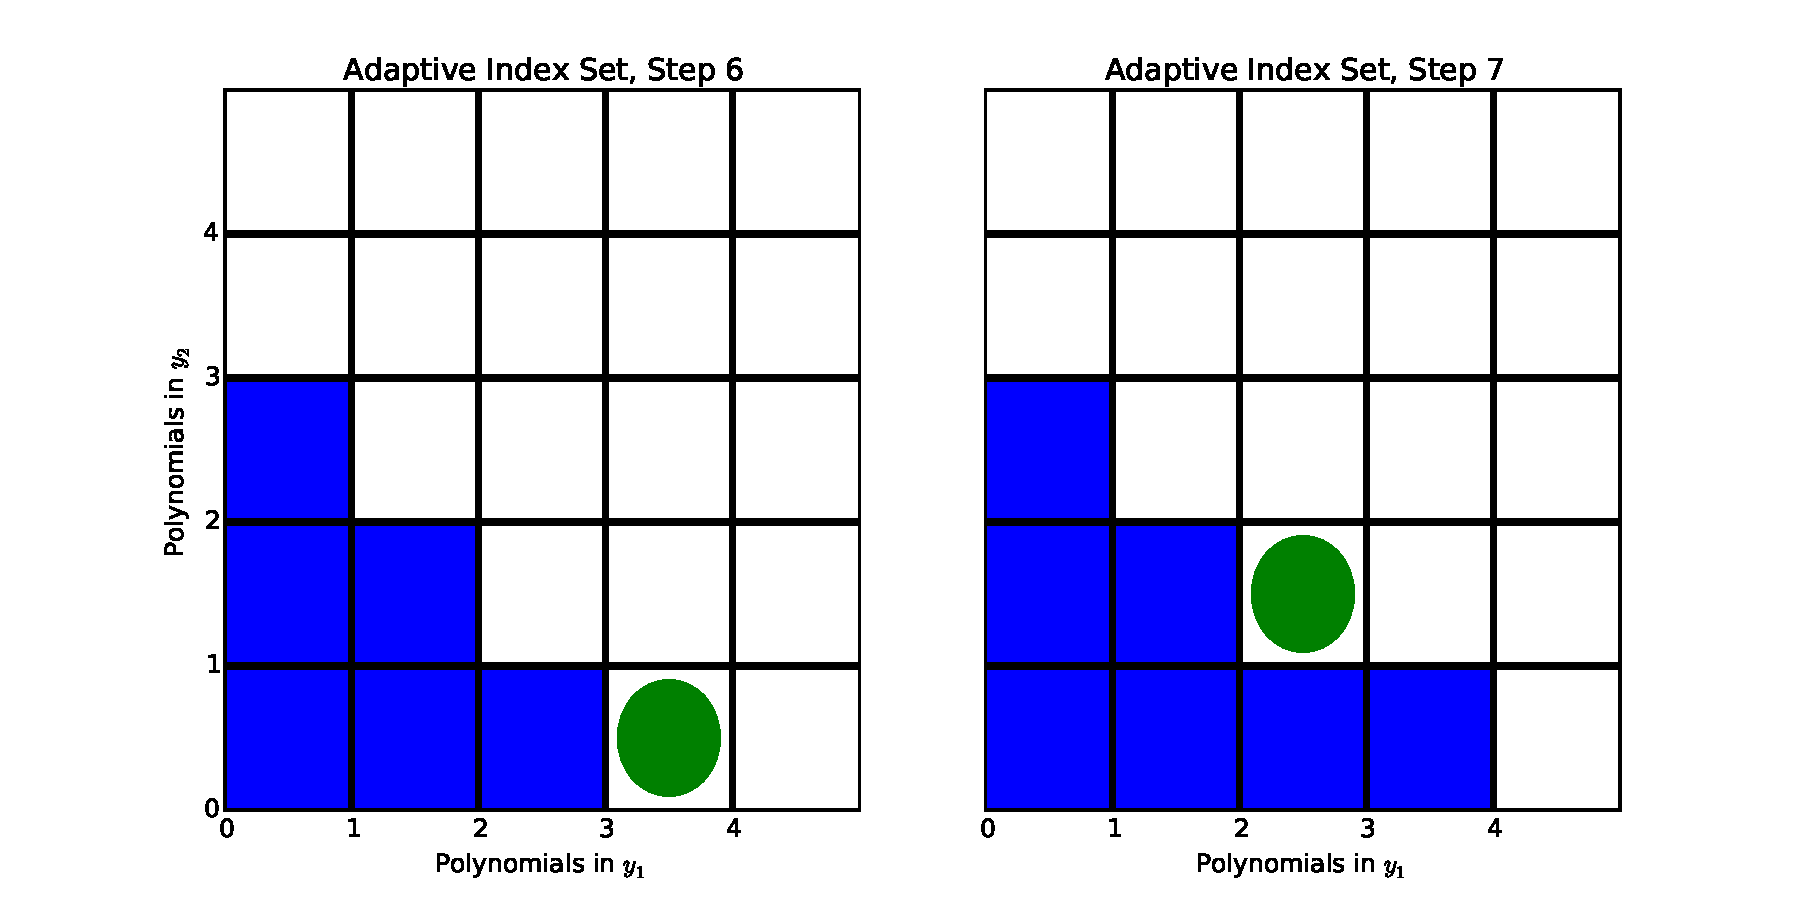
\includegraphics[width=\linewidth]{asc_step}
  \caption{Adaptive Sparse Grid Step}
  \label{fig:asg step}
\end{figure}
\begin{figure}[H]
  \centering
  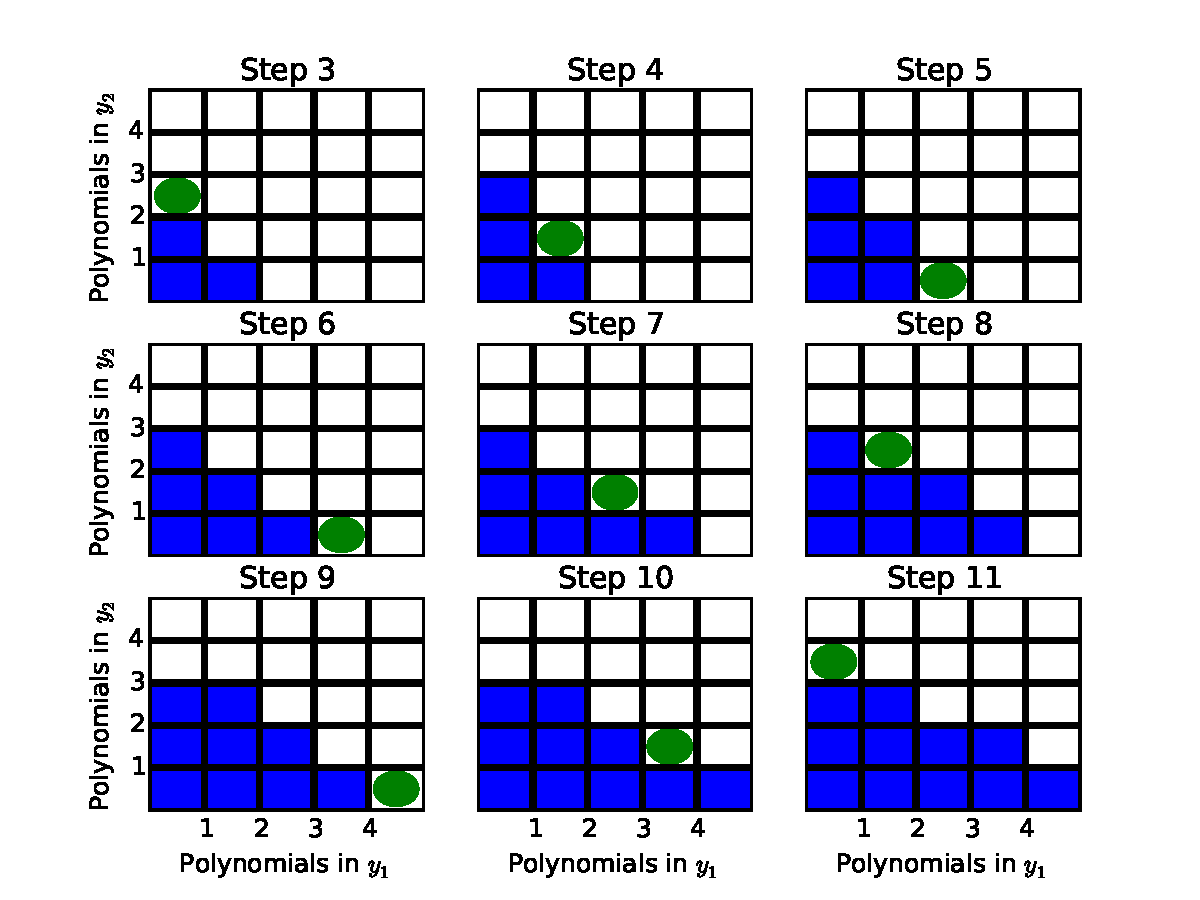
\includegraphics[width=0.7\linewidth]{asc_block}
  \caption{Adaptive Sparse Grid Progression}
  \label{fig:asg block}
\end{figure}

There are, however, some weak points in this algorithm.  First, the current algorithm has no predictive method
to determine the next polynomial index to include in the set in step \ref{item:calc impact} in the adaptive
algorithm above; instead, it evaluates each prospective polynomial and
selects the one with the most impact.  This is somewhat inefficient, because many SCgPC expansion coefficients
that are calculated are not used in the final expansion.  
One improvement we make to this algorithm is to predict the impact of
prospective polynomials based on the impact of predecessors.

In order to predict the most valuable polynomial to add to an expansion during an adaptive search, we first
identify a metric by which different polynomials can be compared to determine impact.  Because our interest 
is in second-order statistics, and the variance of the
polynomial expansions is the sum of the polynomial expansion coefficients, we consider the \emph{impact}
parameter
$\eta_k$ of a polynomial to be the square of its polynomial expansion coefficient,
\begin{equation}\label{eq: act poly impact}
  \eta_k = u_k^2.
\end{equation}
This choice is made because the total variance is the sum of the square of the polynomial expansion
coefficients; therefore, the impact of the square of each polynomial coefficient is also the impact on
the variance.
To estimate the impact of a polynomial whose coefficient is not yet calculated, we consider the average of the
 proceeding polynomials.  That is, for a polynomial $k=(3,2,4)$ we average the impacts of $(2,2,4)$, $(3,1,4)$,
and $(3,1,3)$,
\begin{equation}\label{eq: poly impact}
  \tilde \eta_k = \frac{1}{N-j}\sum_{n=1}^N \eta_{k-e_n},
\end{equation}
where $\tilde \eta_k$ is the estimated impact of polynomial $k$, $e_n$ is a unit vector in dimension $n$, and
for every entry where $k-e_n$ would reduce one index to less than 0, it is skipped and $j$ is incremented by
one.  In this way any polynomial with some missing predecessors is still averaged appropriately with all
available information.  While occasionally this prediction algorithm may be misled, in general it saves
many evaluations over the previous algorithm.

Another weakness of the adaptive sparse grid algorithm is that 
there are certain types of models for which the adaptive algorithm will stall, converge too early, or
similarly fail.  For instance, if the partial derivative of the model with respect to any of the
input dimensions is zero when evaluated at the mean point (but nonzero elsewhere), the algorithm will falsely
converge prematurely, as adding additional polynomial orders to the input in question will not change the
value of the model at the mean point.

For example, consider a model
\begin{equation}
  f(a,b) = a^3b^3,
\end{equation}
with both $a$ and $b$ uniformly distributed on [-1,1].  We note the partial derivatives with respect to either
input variable evaluated at the central point $k=(0,0)$ are zero.  The first polynomial index set point to
evaluate is zeroth-order quadrature in each dimension, $\hat L_k=(0,0)$.
The quadrature point to
evaluate this polynomial coefficient is $Y_\omega=(0,0)$, which, when evaluated, gives $f(0,0)=0$.  

The next polynomial
index set combinations are $k=(0,1)$ and $k=(1,0)$.  For $k=(0,1)$, the quadrature points required are
$Y_\omega=(0,\pm\sqrt{1/3})$.  This evaluates to $f(0,\pm\sqrt{1/3})=0$, as well.  Because of model symmetry, we obtain the
same result for $k=(1,0)$.  According to our algorithm, because our old value was 0, and the sum of the new
contributions is 0, we have converged; however, we know this is false convergence.  

While we expect few
applications for SCgPC to exhibit these zero partial derivatives in the input space, it is a limitation to
consider.  An argument can be made that, since lower-order polynomials correspond to lower-energy modes of the
modeled physics, it is expected that higher-order polynomials should not often contribute to an accurate
expansion unless lower-order polynomials contribute as well.
